En este capítulo se analizarán los problemas que tiene la manera en la que se maneja actualmente la clínica y el por qué es necesario el sistema para agilizar determinados procesos, así como las alternativas de solución que se proponen y cuál de éstas es la que mejor resuelve la problemática. \\

También se tratarán los actores dentro del sistema actual y cómo se manejarán dentro de nuestro sistema. Se describe la problemática y los problemas puntuales encontrados, desglosados por el diagrama de Ishikawa para profundizarlos y resolverlos.

%--------------------------------------------------
\section{Contexto del sistema}

En una cl\'inica que cuenta con 12 consultorios se brindan los servicios de consultas m\'edicas y farmacia.

Actualmente la agendaci\'on de citas es mediante una llamada telef\o'nica, o bien, asistiendo a la cl\'inica para solicitar dicha cita. Se toman los datos del paciente, se reserva una hora dada y estos datos se apuntan en una agenda junto con la informaci\'on del m\'edico que dar\'a la consulta.

Los expedientes cl\'inicos se almacenan en una zona donde se mantienen en un archivador  ordenados alfab\'eticamente y contenidos en un folder.
Las recetas y/o tratamientos indicados por los m\'edicos se escriben a mano y se genera la copia mediante papel carb\'on, una copia para el expediente y otra para el paciente.

En un documento se lleva un registro del inventario de la farmacia, el farmac\'eutico lo almacena en una carpeta.

Diariamente se realiza un cierre de caja y se registra el dinero que ingreso como pago de consultas as\'i como de las ventas de la farmacia, estas cantidades se registran a mano y se archivan. Para corroborar que el dinero corresponda a las consultas otorgadas se tiene que comparar el registro obtenido en el cierre con el registro de las citas pagadas ese d\'ia y el inventario de la farmacia.

%--------------------------------------------------
\section{Procesos actuales}

% - - - - - - - - - - - - - - - - - - - - - - - - -
\subsection{Participantes}

Nombre: Caja.

Descrición: La caja es una zona dentro de la clínica donde las personas van a pagar fichas de consultas.

Responsabilidades: La caja se encarga de cobrar las citas, de cobrar las recetas médicas y cualquier cosa que se requiera durante una cita como aplicaciones de inyecciones o chequeo de la presión. \\

Nombre: Médico.

Descripción: El médico es la persona que se encuentra dentro de un consultorio donde los pacientes son atendidos.

Responsabilidades: Registrar consultas, generar recetas médicas de los pacientes, revisar que la consulta que se está atendiendo está en el sistema y modificar expedientes. \\

Nombre: Cliente.

Descripción: El cliente es la persona que asiste a una cita que haya agendado en caso de estar enfermo y es checado por el médico.

Responsabilidades: Dar de alta su cita en el sistema, asistir a su cita puntual, solicitar mover su cita en caso de no poder asistir el día agendado, tomar el medicamento que le receten y asistir a chequeos en caso de necesitarlos. \\

Nombre: Recepción.

Descripción: La recepción es la zona de la clínica que recibe a los clientes.

Responsabilidades: Recibir a los pacientes, checar que la cita solicitada está en el sistema, dar la ficha de cita a los pacientes para que puedan pagar en caja, agendar citas de manera presencial y mover citas de forma presencial. \\

Nombre: Expediente.

Descripción: El expediente es un documento que contiene toda la información clínica sobre un paciente.

Responsabilidades: Almacenar la información de los pacientes. \\

Nombre: Administrador.

Descripción: El administrador es la persona encargada de mantener al sistema y de evitar irregularidades en éste.

Responsabilidades: Dar de alta o de baja médicos, encargados de farmacia y medicamentos. \\

% - - - - - - - - - - - - - - - - - - - - - - - - -
\subsection{Procesos}

diagramas y explicación de los procesos: describir las actividades.

%--------------------------------------------------
\section{Problemas identificados}

% - - - - - - - - - - - - - - - - - - - - - - - - -
\subsection{Problema general}

La forma de almacenar los expedientes provoca que su consulta sea tardada y se da\~nen con el paso del tiempo.
 
Los tel\'efonos para agendar una cita son limitados, por lo que pueden estar ocupados a la hora de querer agendar una cita; agendar la cita personalmente puede tomar bastante tiempo, desde el traslado hasta si hay otras personas esperando agendar una cita. 

El proceso para recorrer su cita puede llegar a ser tardado.

Dos citas pueden terminar agendadas para una misma fecha y hora, y el chequeo para evitar esto puede tomar mucho tiempo.

En la elaboraci\'on de recetas, el revisar el historial cl\'inico de una persona para poder darle el medicamento adecuado, revisar los registros de recetas y tratamientos anteriores, generar una copia de la receta y otra para el paciente es tardado y usa tiempo que puede usarse para consulta.

El proceso de manejo de la caja puede ser muy tardado y es propenso a errores.

% - - - - - - - - - - - - - - - - - - - - - - - - -
\subsection{Descomposición del problema}

1. La generación de citas se hace de manera ineficiente al usar solo 2 teléfonos y de manera presencial de igual forma es ineficiente al poder tener al recepcionista ocupado con una llamada o generando la cita de alguien más. \\

2. Los expedientes se maltratan debido a que son de papel y aún en un folder al consultarlos se deteriora el material y se puede perder información. \\

3. Mover una cita es ineficiente ya que el registro se lleva en una agenda y para moverlas se debe borrar de la hoja donde está escrita y reescribirla en la nueva fecha, pero esto maltrata la hoja donde se escribió antes. \\

4. El atender a un paciente puede tomar demasiado tiempo por la consulta de su expediente, ya que se debe buscar por orden alfabético donde está en caso de tener ya un expediente generado. \\

5. Existe un alto riesgo de agendar dos citas a la misma hora el mismo día y en el mismo consultorio debido a la forma en la que se agendan citas actualmente. \\

6. La creación de recetas es de manera ineficiente y se pueden perder recetas de pacientes debido a que si un paciente va demasiadas veces a consulta y genera muchas recetas en un folder podrían salirse. \\

7. La consulta de recetas también es de manera tardada ya que para checar qué se ha recetado en un período de tiempo se deben buscar todos los registros y checarlos uno por uno y puede tardar. \\

8. Al cierre de caja es muy pesado checar en la caja lo que se vendió de forma manual y todavía checar el inventario para ver que corresponda con lo vendido. \\

9. Al cierre de caja es pesado checar cada consultorio si las citas escritas en la agenda corresponden con las atendidas. \\

10. La entrada de cada doctor es de manera irregular ya que el hecho de que solo exista un checador y que dos doctores entren al mismo tiempo hace que una entrada se registre después de otra y si eso fuese perder un minuto en el chequeo al doctor que checó después se le puede acumular como retraso.

% - - - - - - - - - - - - - - - - - - - - - - - - -
\subsection{Análisis de causas}

\begin{center}
\fbox{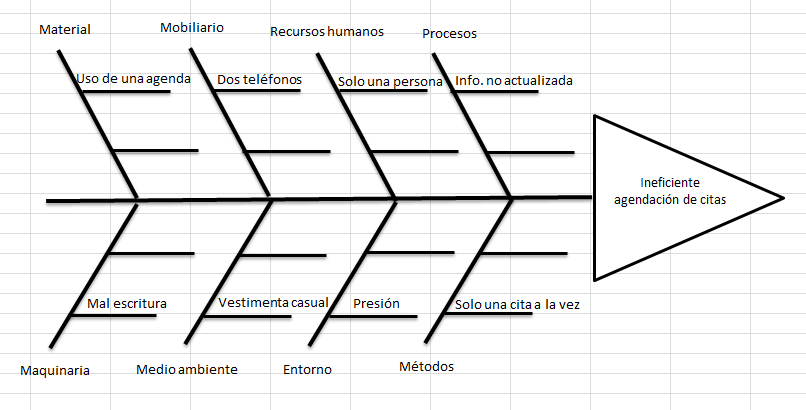
\includegraphics[width=16cm,height=8cm]{images/Ishikawa1.PNG}}
\end{center}

%--------------------------------------------------
\section{Propuesta de solución}

% - - - - - - - - - - - - - - - - - - - - - - - - -
\subsection{Alternativas de solución}

1. Crear un sistema local para crear citas y almacenar expedientes en un ordenador como servidor que se conecte al resto de los ordenadores. \\

2. Almacenar los expedientes en un sistema de archivos y comprar más teléfonos y contratar más personas para poder atender la mayor cantidad de citas posibles. \\

3. Crear un sistema con plataforma web para el registro de citas, la consulta de expedientes de forma local desde las computadoras dentro de la clínica y el registro de recetas médicas. \\

4. Crear un sistema que permita la generación de citas vía web, un sistema de archivos para los expedientes y recetas y una plataforma para el acceso de dichos sistemas de archivos. \\

5. Colocar un límite en la cantidad de citas por día para evitar el sobrepedido y guardar los expedientes en un almacén especial para ellos.
